\documentclass[12pt, letterpaper, preprint, tighten]{aastex}
\usepackage[breaklinks,colorlinks, urlcolor=blue,citecolor=blue,linkcolor=blue]{hyperref}
\usepackage{amsmath}
%\usepackage{hyperref}
%\usepackage{cite}
\usepackage{color}
\usepackage{comment}
%%% This file is generated by the Makefile.
\newcommand{\giturl}{\url{https://github.com/changhoonhahn/centralMS}}
\newcommand{\githash}{9119283}\newcommand{\gitdate}{2019-04-05}\newcommand{\gitauthor}{changhoonhahn}


% typesetting shih
\linespread{1.08} % close to 10/13 spacing
\setlength{\parindent}{1.08\baselineskip} % Bringhurst
\setlength{\parskip}{0ex}
\let\oldbibliography\thebibliography % killin' me.
\renewcommand{\thebibliography}[1]{%
  \oldbibliography{#1}%
  \setlength{\itemsep}{0pt}%
  \setlength{\parsep}{0pt}%
  \setlength{\parskip}{0pt}%
  \setlength{\bibsep}{0ex}
  \raggedright
}
\setlength{\footnotesep}{0ex} % seriously?

\newcommand\tab[1][1cm]{\hspace*{#1}}
\newcommand{\todo}[1]{{\bf \textcolor{red}{#1}}}
\newcommand{\beq}{\begin{equation}}
\newcommand{\eeq}{\end{equation}}
\newcommand{\overbar}[1]{\mkern 1.5mu\overline{\mkern-1.5mu#1\mkern-1.5mu}\mkern 1.5mu}
\newcommand{\avgSFR}{\overline{\raisebox{0pt}[1.2\height]{SFR}}}
\newcommand{\SFR}{\mathrm{SFR}}
\newcommand{\fq}{f_\mathrm{Q}}
\newcommand{\fqcen}{f_\mathrm{Q}^\mathrm{cen}}
\newcommand{\zinit}{z_\mathrm{initial}}
\newcommand{\taucen}{\tau_\mathrm{Q}^\mathrm{cen}}
\newcommand{\logsfr}{\log \, \mathrm{SFR}}
\newcommand{\bitem}{\begin{itemize}}
\newcommand{\eitem}{\end{itemize}}
\newcommand{\musfms}{\log\,\overline{\mathrm{SFR}}_\mathrm{SFS}}
\newcommand{\siglogm}{\sigma_{\log\,M_*}} 
\newcommand{\hahngmm}{Hahn et al. (in prep.)} 

\begin{document}\sloppy\sloppypar\frenchspacing

\title{Star Formation Sequence in a Hierarchical Universe} 
%\title{Central Galaxies on the Main Sequence} 
\date{\texttt{DRAFT~---~\githash~---~\gitdate~---~NOT READY FOR DISTRIBUTION}}
\author{ChangHoon~Hahn\altaffilmark{1, 2}, 
Jeremy L.~Tinker\altaffilmark{2}, 
Andrew R.~Wetzel\altaffilmark{3,4,5}}
\altaffiltext{1}{Lawrence Berkeley National Laboratory, 1 Cyclotron Road, Berkeley, CA 94720}
\altaffiltext{2}{Center for Cosmology and Particle Physics, Department of Physics, New York University, 4 Washington Place, New York, NY 10003}
\altaffiltext{3}{TAPIR, California Institute of Technology, Pasadena, CA USA}
\altaffiltext{4}{Carnegie Observatories, Pasadena, CA USA}
\altaffiltext{5}{Department of Physics, University of California, Davis, CA USA}
\email{changhoon.hahn@lbl.gov}

\begin{abstract}
    \todo{motivation, methodology, impact.}
    In observations star forming galaxies form a tight $log\;M_*$ to $log\;SFR$ 
    relation referred to as the {\em star formation main sequence} (SFS) out to $z\sim2$. 
    Beyond the evolution ``along'' this SFS, however, the star formation histories of star 
    forming galaxies have not been precisely characterized. 
    The SFH of these galaxies govern SMF, SFS, and also observed constraints on the stellar mass to halo mass
    relation. 

    By combining high-resolution cosmological $N$-body simulation with observed evolutionary 
    trends of SF galaxies, we construct a model that tracks the evolution of star forming 
    central galaxies over the redshift $z < 1$. Comparing this model 

    Observations find a remarkably small scatter in the stellar mass to halo mass relation. 
    Somehow the star formation histories of galaxies must 
    
    According to observations, star forming galaxies form a tight $log\;M_*$ to $log\;SFR$ 
    relation referred to as the ``star formation main sequence'' out to $z\sim2$. 
\end{abstract}
\keywords{methods: numerical -- galaxies: clusters: general -- 
galaxies: groups: general -- galaxies: evolution -- galaxies: haloes -- 
galaxies: star formation -- cosmology: observations.}

\section{Introduction}
\bitem 
\item Motivate why we think SF galaxies evolve along the main sequence  
\item Discuss the current thought process on galaxy assembly bias 
\item Explain the limitation of SFH derivable from observations (Claire's fisher matrix paper would be really good; ask her about the details) 
\item in fact we can't constrain sf variability very well even in simulations due to the time resolution (see \hahngmm).  
\item Observations also can't provide detail host dark matter halo properties
\item So the approach with combining observations with N-body (empirical modeling) is very effective in the context of the halo.
\item Maybe talk about how the bigger context of why this is important?  
\item Why only centrals -- because our current best understanding of satellites is that they quench after infall, so it doesn't make sense to look at them
\item our model goes from $z < 1$ because beyond that the observations are statistically meaningless.  
\eitem 

%%%%%%%%%%%%%%%%%%%%%%%%%%%%%%%%%%%%%
% Figure 1 
%%%%%%%%%%%%%%%%%%%%%%%%%%%%%%%%%%%%%
\begin{figure}
\begin{center}
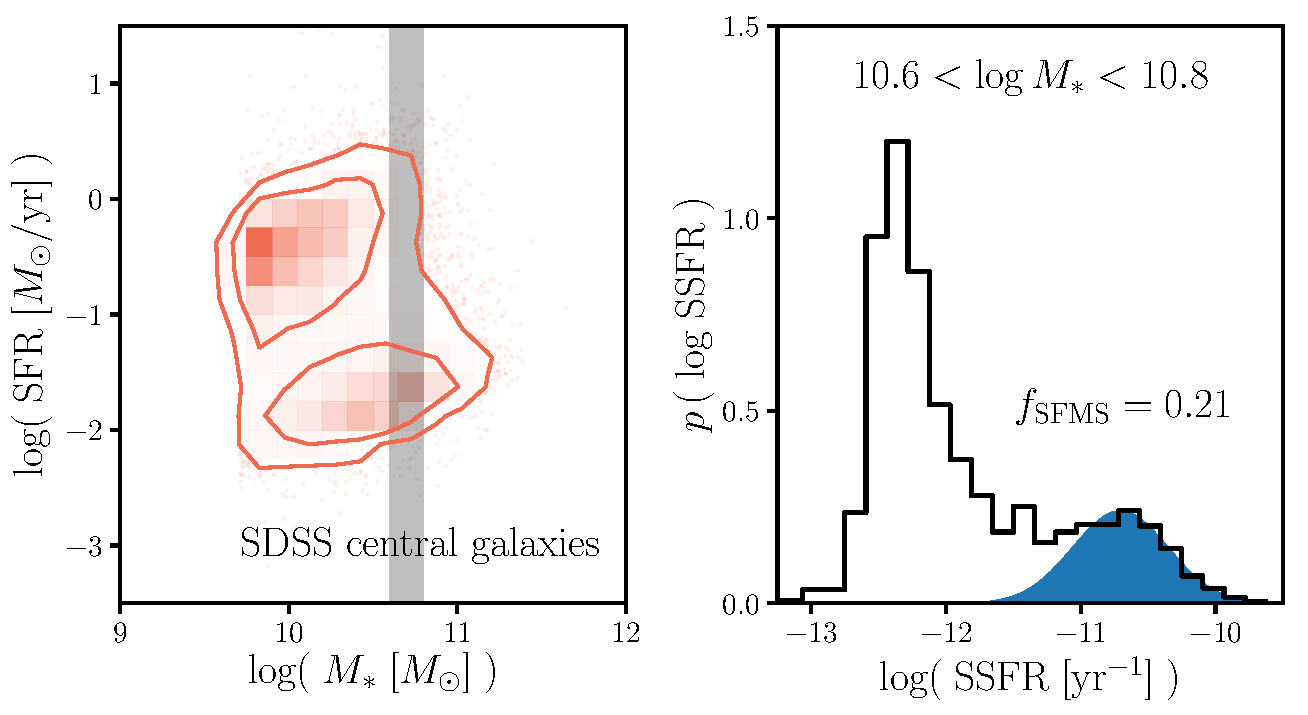
\includegraphics[width=0.75\textwidth]{figs/groupcat.pdf}
    \caption{Central galaxies of the SDSS DR7 group catalog. \emph{Left:} We plot 
    the SFR-$M_*$ relation of the SDSS central galaxies. The contours illustrate the bimodal
    distribution of the galaxy properties and mark the star-forming and quiescent populations. 
    The transitioning galaxies lie on the ``green'' valley between the star-fomring and quiescent
    modes. %The dashed line represents the linear fit to the SFS as described in Section~\ref{sec:sfcen}. 
    \emph{Right:} We plot the distribution of $\mathrm{log}\,\mathrm{SSFR}$ for SDSS centrals
    with $10.6 < \mathrm{log}\,M_* < 10.8$. Shaded in blue, we plot the SFS component of our 
    GMM fit of the SFR-$M_*$ relation described in Section~\ref{sec:sfcen}. Based on this fit, 
    galaxies in the SFS account for approximately $f_\mathrm{SFS} = 0.21$ of the central 
    galaxies in the stellar mass bin.} \label{fig:groupcat}
\end{center}
\end{figure}
%%%%%%%%%%%%%%%%%%%%%%%%%%%%%%%%%%%%%

\section{Central Galaxies of SDSS DR7} \label{sec:sdss}
We construct our galaxy sample following the sample selection of \cite{tinker2011}. 
We select a volume-limited sample of galaxies with $M_r −5 log(h) < −18$ and complete in
$M_* > 10^{9.4} M_\odot$ from the NYU Value-Added Galaxy Catalog \citep[VAGC;][]{blanton2005}
of the Sloan Digital Sky Survey Data Release 7~\citep[SDSS DR7;][]{abazajian2009} at 
$z \approx 0.04$. The stellar masses of these galaxies are estimated using the
$\mathtt{kcorrect}$ code~\citep{blanton2007} assuming a~\cite{chabrier2003} initial
mass function. The star formation of the galaxies are estimated spectroscopically using the
specific star formation rates (SSFR) from the current release of the MPA-JHU spectral 
reductions\footnote{http://wwwmpa.mpa-garching.mpg.de/SDSS/DR7/}~\citep{brinchmann2004}.
Generally speaking, $\mathrm{SSFR} > 10^{-11}\mathrm{yr}^{-1}$ are derived from 
$\mathrm{H}_\alpha$ emission, $10^{-11} > \mathrm{SSFR} > 10^{-12}\mathrm{yr}^{-1}$
are derived from a combination of emission lines, and $\mathrm{SSFR} < 10^{-12}\mathrm{yr}^{-1}$
are based on $D_n 4000$~\citep[see discussion in][]{wetzel2013}. We note that 
$\mathrm{SSFR} < 10^{-12}\mathrm{yr}^{-1}$ should only be considered upper limits 
to the true galaxy SSFR~\citep{salim2007}.

From our galaxy sample, we identify the central galaxies using the \cite{tinker2011} halo-based 
group-finding algorithm, which is based on the~\cite{yang2005} algorithm and tested 
in~\cite{campbell2015}. The algorithm assigns a probability of being a satellite,
$P_\mathrm{sat}$, to each galaxy in the sample. Galaxies with $P_\mathrm{sat} \geq 0.5$ 
are classified as satellites and $P_\mathrm{sat} < 0.5$ are classified as centrals. 
In this paper we focus on central galaxies. With any group finding algorithm, galaxies are 
misassigned due to projection effects and redshift space distortions. The purity 
of the full central galaxy sample is $\sim 90\%$ with a completeness of $\sim 95\%$~\citep{tinker2017}.
Furthermore, \cite{campbell2015} find that the algorithm robustly identifies red and blue centrals
as a function of stellar mass, which is highly relevant to our analysis.  

In the left panel of Figure~\ref{fig:groupcat}, we plot the SFR-$M_*$ distribution of
the SDSS DR7 central galaxies. In the right panel, we plot the distribution of SSFR, 
$p(\log \mathrm{SSFR})$, for galaxies with $10.6 < \log \,M_* < 10.8$ (stellar mass range 
highlighted on the left panel). Both panels of Figure~\ref{fig:groupcat} illustrate the 
bimodality in the galaxy sample. The SFR-$M_*$ distribution also illustrate the correlation
between SFR and $M_*$ in star-forming galaxies \emph{i.e.} the star-formation main sequence 
(SFS).

\section{Model: Simulated Central Galaxies} \label{sec:sim}
We're interesting in constructing a model that tracks central galaxies and 
their star formation within the heirarchical growth of their host halos. This 
requires a cosmological $N$-body simulation that accounts for the complex 
dynamical processes that govern the host halos of galaxies. In this paper 
we use the high resolution $N$-body simulation from~\cite{wetzel2013} generated 
using the \cite{white2002} $\mathtt{TreePM}$ code with flat $\Lambda$CDM cosmology 
($\Omega_m =0.274, \Omega_b = 0.0457, h = 0.7, n=0.95, \mathrm{and} \sigma_8 = 0.8$).
From initial conditions at $z = 150$ generated from second-order Lagrangian 
Perturbation Theory, $2048^3$ particles with mass of $1.98 \times 10^8\,M_\odot$ are 
evolved in a $250 \mathrm{Mpc}/h$ box with a Plummer equivalent smoothing of 
$2.5\,\mathrm{kpc}/h$. For a more detailed description of the simulation, we 
refer readers to~\cite{wetzel2013, wetzel2014}.

From the $\mathrm{TreePM}$ $N$-body simulation, `host halos' are identified 
using the Friends-of-Friends (FoF) algorithm of \cite{davis1985} with 
linking length of $b = 0.168$ times the mean inter-partcile spacing. Within 
these host halos, \cite{wetzel2013} identifies `subhalos' as overdensities 
in phase space through a six-dimensional FoF algorithm~\citep[FoF6D][]{white2010}. 
The host halos and subhalos are then tracked across the simulation outputs 
from $z = 10$ to $0$ to build merger trees~\citep{wetzel2009,wetzel2010}. 
The most massive subhalos in newly-formed host halos at a given simulation 
output are defined as the `central' subhalo. A central subhalo retains its 
`central' definition until it falls into a more massive host halo, at which 
point it becomes a `satellite' subhalo. 

At a given snapshot, we assign stellar masses used only for initializing
our model to each subhalo by subhalo abundance matching~\citep[SHAM;][]{conroy2006,vale2006,yang2009,wetzel2012,leja2013,wetzel2013,wetzel2014,hahn2017a}
to $M_\mathrm{peak}$, the maxmum host halo mass that it ever had as a 
central subhalo. SHAM, in its simplest form, assumes a one-to-one mapping 
between subhalo $M_\mathrm{peak}$ and galaxy stellar mass $M_*$ that 
preserves rank order: $n(> M_\mathrm{peak}) > n(> M_*)$. In practice, we 
apply a $0.2$ dex log-normal scatter in $M_∗$ at fixed $M_\mathrm{peak}$ 
based on the observed stellar to halo mass relation (SHMR; \todo{bunch of SMHMR citations}). %\cite{gu2016} compile empirical constraints on the scatter of this stellar mass to halo mass relation ($\sigma_{\log M_*}$). 
For $n(> M_*)$, we use observed stellar mass functions (SMFs) at the redshift 
corresponding to the snapshot. At $z=0.05$, the lowest redshift snapshot of 
our model, we use the SMF from \cite{li2009}, which is based on the same 
SDSS NYU-VAGC sample as our group catalog. At higher redshifts, we interpolate 
between the \cite{li2009} SMF and the SMF from \cite{marchesini2009} at 
$z = 1.6$. We choose the \cite{marchesini2009} SMF, among others, because it 
produces interpolated SMFs that monotonically increase at $z < 1$. As noted 
in \cite{hahn2017a}, at $z \approx 1$, the SMF interpolated between the 
\cite{li2009} and \cite{marchesini2009} SMFs is consistent with more recent 
measurements from \cite{muzzin2013} and \cite{ilbert2013}. 
\todo{TBD: Perhaps mention in appendix how we test different SMF assumptions}% (In Section~\ref{app:z1},)

Throughout its $45$ snapshot outs, $\mathtt{TreePM}$ simulation tracks 
the evolution of subhalos back to $z \sim 10$. We restrict ourselves to $15$ 
snapshots from $z = 1.08$ to $z=0.05$, where we have the most statistically 
meaningful observations. Furthermore, since we're interested in centrals we only 
keep subhalos that are classified as centrals throughout the redshift 
range. This criterion removes ``black splash'' or ``ejected'' satellite 
galaxies~\citep[\emph{e.g.}][]{mamon2004,wetzel2014} misclassified as 
centrals. Finally, we have a model based on the $\mathtt{TreePM}$ $N$-body 
simulation that tracks the evolution of central subhalos from $z = 1.08$ to 
$z=0.05$. Next, we describe how we select and initialize the star forming 
central galaxies from the central subhalos in our model. 

%%%%%%%%%%%%%%%%%%%%%%%%%%%%%%%%%%%%%
% Figure 2 
%%%%%%%%%%%%%%%%%%%%%%%%%%%%%%%%%%%%%
%\begin{figure}
%\begin{center}
%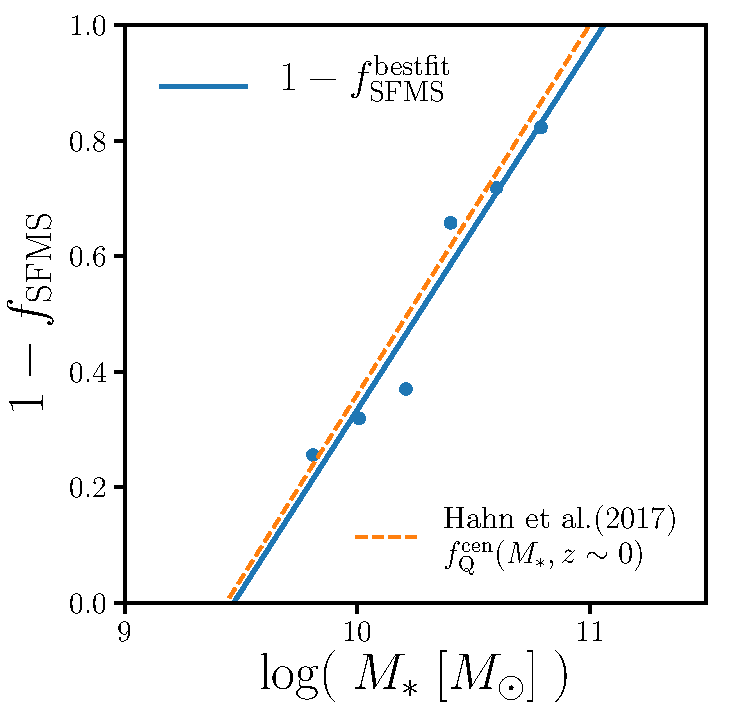
\includegraphics[width=0.5\textwidth]{figs/fq_fsfms.pdf}
%\caption{SFS fraction versus quiescent fraction from Hahn}
%\label{fig:fq_fsfms}
%\end{center}
%\end{figure}
%%%%%%%%%%%%%%%%%%%%%%%%%%%%%%%%%%%%%

\subsection{Selecting Star Forming Centrals}  \label{sec:sfcen}
In our model, we're interested in tracking the SFR and stellar mass 
evolution of SF central galaxies. To construct such a model, we 
first need to select SF galaxies from the central galaxies in our 
simulation, described above. Since we want our model to reproduce 
observations, our selection is based on $f^\mathrm{cen}_\mathrm{SFS}(M_*)$, 
the fraction of central galaxies within the star forming sequence, 
measured from the SDSS DR7 VAGC (Section~\ref{sec:sdss}). Below, we 
describe how we derive this $f^\mathrm{cen}_\mathrm{SFS}(M_*)$ and use 
it to select SF central galaxies in our model. Afterwards we describe how 
we initalize the SFRs and $M_*$ of these galaxies in our model.

Often in the literature, an empirical color-color or SFR--$M_*$ cut 
that separates the two main modes (red/blue or star-forming/quiescent) 
in the distribution is chosen to classify 
galaxies~\citep[\emph{e.g.}][]{baldry2006, blanton2009, drory2009, peng2010, moustakas2013, hahn2015}.
The red/quiescent or blue/star-forming fractions derived from this sort 
of classification, by construction, depend on the choice of cut and 
neglect galaxy subpopulations such as transitioning galaxies~\emph{i.e.} 
galaxies in the ``green valley''. Instead, for our 
$f^\mathrm{cen}_\mathrm{SFS}(M_*)$, we use the SFS fitting method 
from \hahngmm. \hahngmm uses Gaussian Mixture Models and the Bayesian 
Information Criteria in order to fit the SFR--$M_*$ relation of a galaxy 
population and identify its SFS. This data-driven approach relaxes 
many of the assumptions and hard cuts that go into other methods. 
Furthermore, as they demonstrate in \hahngmm by applying to multiple 
simulations, it can be flexibly applied to a wide range of star 
formation and $M_*$. The weight of the SFS GMM component from the 
fitting provides an estimate of $f^\mathrm{cen}_\mathrm{SFS}$. 
In the right panel of Figure~\ref{fig:groupcat}, we plot the SFS 
GMM component (blue shaded region) of the $p(\log \mathrm{SSFR})$ 
for the SDSS DR7 central galaxies within $10.6 < \log M_* < 10.8$. 
The SFS constitutes $f^\mathrm{cen}_\mathrm{SFS} = 0.21$ of the 
SDSS central galaxies in this stellar mass bin. 

%we instead use a method from \todo{Hahn et al.~(in prep)} and Tjitske et 
%al.~(in prep), which is a data-driven fitting of the SFS from the SFR-$M_*$ 
%distribution using Gaussian Mixture Models (GMMs). 
%Using the Hahn et al.~(in prep) SFS fitting, we fit the SSFR 
%distributions of the SDSS DR7 VAGC centrals in $\log\,M_*$ bins 
%of width $0.2~\mathrm{dex}$ using GMMs with $k = 1 - 3$ components 
%using the expectation-maximization 
%algorithm~\citep[EM;][]{dempster1977, neal1998}. We restrict 
%ourselves to models with a maximum of $3$ components for the three 
%possible galaxy classifications: quiescent, SF, and transitioning populations. From the three GMMs, we select the model with 
%the lowest Bayesian Information Criteria~\citep[BIC;][]{schwarz1978}. 
%The Gaussian component of this GMM with mean $\log \mathrm{SSFR} > -11$ 
%is identified as the SFS. In the rare cases when more than one GMM 
%component has mean $\log \mathrm{SSFR} > -11$, we compare the weights 
%of the components.  If the weight of one component is less than a 
%third of the other, we take the component with the higher weight to 
%represent the SFS. Otherwise, we omit the stellar mass bin altogether. 
%\todo{sentence about how for the VAGC, we don't omit any stellar mass bins} 

Rather than using the $f^\mathrm{cen}_\mathrm{SFS}$ values directly, 
for selecting SF galaxies, we fit $f^\mathrm{cen}_\mathrm{SFS}$ as 
a linear function of $\log\,M_*$ similar to \cite{wetzel2013,hahn2017}. 
We derive the following best-fit: 
\beq \label{eq:f_cen_sfms}
f^\mathrm{cen}_\mathrm{SFS, bestfit}(M_*) = -0.627\,(\log\,M_* - 10.5) + 0.354. 
\eeq
We note that this $f^\mathrm{cen}_\mathrm{SFS, bestfit}(M_*)$ is in good 
agreement with the $f_\mathrm{Q}^\mathrm{cen}(M_*; z\sim0)$ fit from 
\cite{hahn2017a}. For each central galaxy in our simulation, we assign 
a probability of it being on the SFS, using Eq.~\ref{eq:f_cen_sfms} 
with $M_*$ at $z \sim 0$ assigned through SHAM. Based on these 
probablities, we randomly identify centrals from our simulation as SF at 
$z \sim 0$. In our model, we make the assumption that once a SF galaxy 
quenches its star formation, it remains quiescent.  %\todo{maybe something about rejuvenation?} 
Without any quiescent galaxies rejuvenating their star formation, galaxies
on the SFS at $z\sim0$ are also on the SFS at $z > 0$. Using this assumption
the SF centrals we select at $z \sim 0$ are also on the SFS at the intial
redshift of our model: $z \sim 1$. 

Next, we can initialize the SF centrals at $z\sim1$ using SHAM $M_*$s and 
assign their initial SFRs based on the observed SFR-$M_*$ relation of the SFS. 
Observations in the literature at these redshifts, however, not only use 
galaxy properties derived differently from the SDSS VAGC but they also 
find SFS with significant discrepancies from one another. \cite{speagle2014} 
compiles the SFR-$M_*$ relation of the SFS from 25 studies in the literature, 
each with different methods of deriving galaxy properties. Even \emph{after} 
their calibration, for a fixed $M_* = 10^{10.5}\, M_\odot$, the SFRs of the 
SFSs at $z \sim 1$ vary by more than a factor of 2~\citep[see Figure 2 of][]{speagle2014}. 
With little consensus on the SFS at $z\sim1$, and consequently its redshift
evolution, we flexibly parameterize the SFS SFR ($\log\,\mathrm{SFR}_\mathrm{MS}(M_*, z)$) 
with free parameters $m_{M_*}$ and $m_z$ that characterize the stellar mass 
and redshift dependences respectively.  %and marginalize over them later in the analysis. 
%This is particularly concerning since the redshift evolution of the SFS dictate the SFR and $M_*$ evolution of SF centrals in our model. 
%So to deal with this uncertainty, we parameterize 
%For our $\log\,\mathrm{SFR}_\mathrm{MS}(M_*, z)$, at $z \sim 0$ we anchor our 
%SFS to the SFS of the SDSS central galaxies, which we obtain from the 
%SFS GMM components used to estimate $f^\mathrm{cen}_\mathrm{SFS}$. Using 
%the mean $\log\, \mathrm{SFR}$ of the SFS GMM component at each stellar 
%mass bin, we linearly fit $\log\, \mathrm{SFR}(M_*)$ (see dashed line in 
%Figure~\ref{fig:groupcat}). Then for $z > 0$, we include two free 
%parameters to account for the redshift evolution of the amplitude and 
%slope of the SFS SFR-$M_*$ relation: $A_z$ and $m_z$, respectively. 
We parameterize the mean $\log\,\mathrm{SFR}$ of the SFS as, 
\beq \label{eq:logsfr_ms}
\log\,\overline{\mathrm{SFR}}_\mathrm{SFS}(M_*, z) =  m_{M_*} * (\log\,M_* - 10.5) + m_z * (z - 0.05) - 0.11.
\eeq
We assign SFRs to our SF centrals at $z\sim1$ by sampling a log-normal 
distribution centered about $\log\,\overline{\mathrm{SFR}}_\mathrm{MS}(M_*, z=1)$ 
with a constant scatter of $0.3\,\mathrm{dex}$, motivated from 
observations~\citep{daddi2007, noeske2007, magdis2012, whitaker2012}.
Later in our analysis, for the priors of our parameters $m_{M_*}$ 
and $m_z$, we conservatively choose a range that encompass the best-fit 
SFS from~\cite{speagle2014} and measurements from~\cite{moustakas2013} 
and~\cite{lee2015}. With our SF centrals initalized at $z \sim 1$, next, 
we describe how we evolve their SFR and $M_*$.

%%%%%%%%%%%%%%%%%%%%%%%%%%%%%%%%%%%%%
% Figure 3 
%%%%%%%%%%%%%%%%%%%%%%%%%%%%%%%%%%%%%
\begin{figure}
\begin{center}
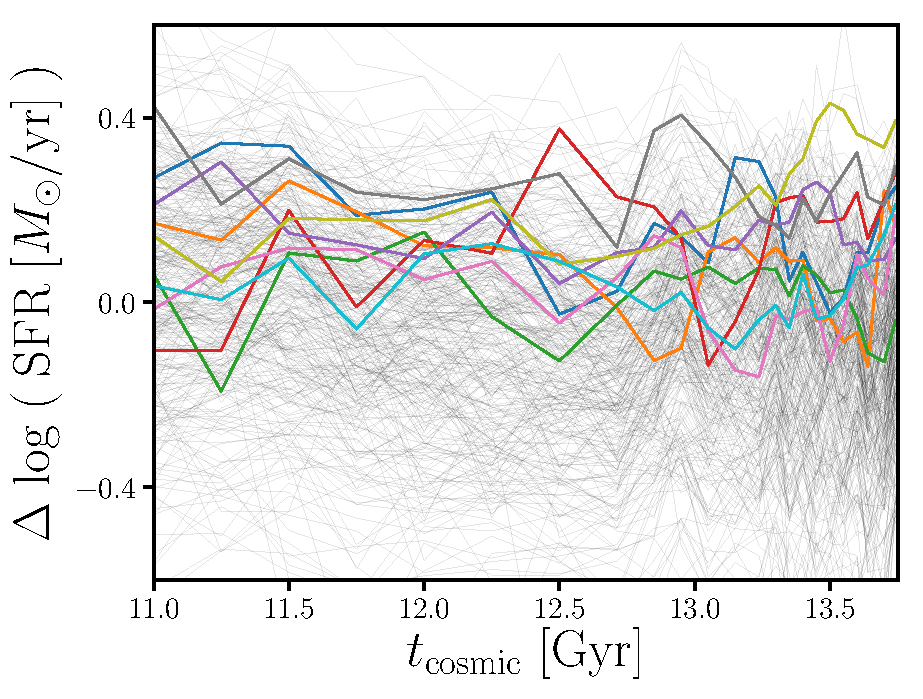
\includegraphics[width=0.5\textwidth]{figs/illustris_sfh.pdf} 
    \caption{Star formation rate with respect to the $\musfms$---$\Delta \logsfr$)---as 
    a function of cosmic time for star-forming galaxies in the Illustris simulation. 
    These galaxies have stellar masses within the range $10^{10.5}-10^{10.6}M_\odot$ 
    at $z\sim0$. $\musfms$ is fit using the \hahngmm SFS fitting method, the same method
    we use for our SDSS centrals in Section~\ref{sec:sfcen}. As the $\Delta \logsfr(t)$s
    in color emphasize how the SFRs of Illustris star-forming galaxies fluctuate about 
    the mean SFS. \emph{The $\mathrm{SFR}$ variability in the SFHs of SF centrals in our model (see 
    Section~\ref{sec:modelevol}) is motivated by this $\Delta \logsfr(t)$ behavior in 
    Illustris.}}
\label{fig:illsfh}
\end{center}
\end{figure}
%%%%%%%%%%%%%%%%%%%%%%%%%%%%%%%%%%%%%

%%%%%%%%%%%%%%%%%%%%%%%%%%%%%%%%%%%%%
% Figure 4 
%%%%%%%%%%%%%%%%%%%%%%%%%%%%%%%%%%%%%
\begin{figure}
\begin{center}
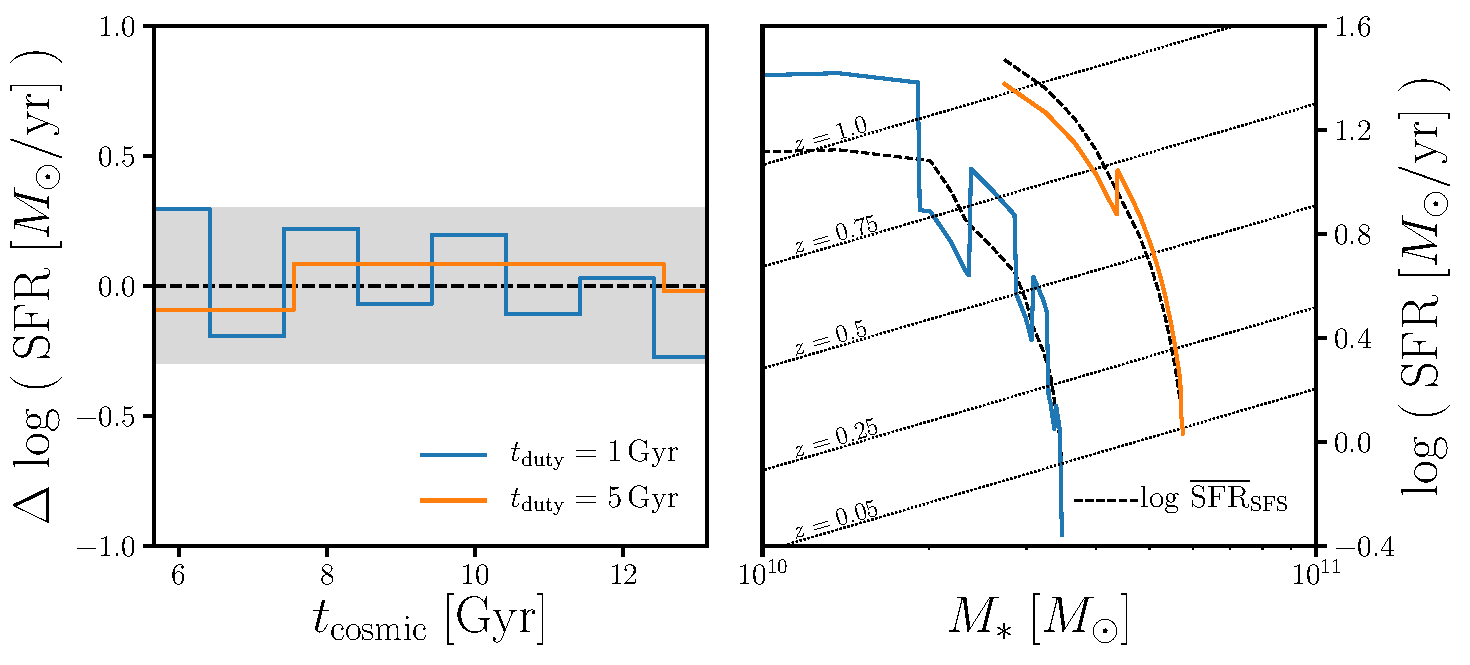
\includegraphics[width=0.9\textwidth]{figs/sfh_pedagogical.pdf}
    \caption{\emph{Left}: The $\Delta \logsfr$ evolution of two SF centrals
    using the fiducial model that incorporates star formation variability through 
    a ``star formation duty cycle'' on two timescales $t_\mathrm{duty} = 1$ Gyr 
    (blue) and $5$ Gyr (orange). $\Delta \logsfr(t)$s determine the SFHs
    (Eq.~\ref{eq:logsfr_sf}), hence it also determines the $M_*$ growth 
    of the SF central galaxies in our model (Eq.~\ref{eq:integ_mass}).  
    \emph{Right}: The $\mathrm{SFR}_i$ and $M_{*,i}$ evolutions of the same two 
    SF central galaxies in our fiducial model with $t_\mathrm{duty} = 1$ Gyr (blue) 
    and $5$ Gyr (orange). For reference we plot $\musfms(M_{*,i}(t), t)$ for 
    each galaxy (black dashed) and $\musfms(M_*)$ at various redshifts between 
    $z = 1$ to $0.05$ (dotted lines). As the $\mathrm{SFR}_i$ and $M_{*,i}$ 
    evolutions illustrate, \emph{the SF centrals in our model evolve as their SFRs 
    fluctate about the SFS.}} \label{fig:sfh_model}
\end{center}
\end{figure}
%%%%%%%%%%%%%%%%%%%%%%%%%%%%%%%%%%%%%


\subsection{Evolving along the Star Formation Sequence} \label{sec:modelevol} 
The tight correlation between the SFRs and stellar masses of SF 
galaxies (the so-called SFS) has been observed to span over four 
orders of magnitude in stellar mass and extends beyond the local 
universe out to $z > 2$ 
(\emph{e.g.}~\citealt{noeske2007,daddi2007,elbaz2007,salim2007,santini2009,karim2011,whitaker2012,moustakas2013,lee2015}; see also references in \citealt{speagle2014}). 
Even in hydrodynamic simulations and semi-analytic models, we find 
well defined SFSs (see \hahngmm and references therein). The SFRs 
of galaxies on the SFS, for a given stellar mass follow a log-normal 
distribution with a roughly constant scatter ($\sim0.3\,\mathrm{dex}$ 
in observations).  %In bins of $\mathrm{log}\,M_*$, the SFRs of galaxies on the SFS are observed to follow a log-normal distribution with a roughly constant scatter of $0.3\,\mathrm{dex}$. 
Given its persistence in the local Universe, the SFS provides a 
anchoring relationship to characterize the SFRs and $M_*$s of SF 
galaxies throughout $z < 1$. More specifically, \emph{we can characterize 
the star formation histories (SFHs) of our SF centrals with respect 
to the mean $\logsfr$ of the SFS} (Eq.~\ref{eq:logsfr_ms}):
\beq \label{eq:logsfr_sf} 
\logsfr(M_*, t) = \log\,\overline{\mathrm{SFR}}_\mathrm{MS}(M_*, t) + \Delta \logsfr(t).
\eeq
Since SFHs determine the $M_*$ growth of galaxies, $\Delta \logsfr$s
in our model dictate the SFHs and $M_*$ evolution of SF centrals. 
Below, we describe the prescription for our fiducial $\Delta \logsfr(t)$.

One naive example for $\Delta \logsfr(t)$ would be to keep 
$\Delta \logsfr$ fixed from the initial offsets from the $\musfms$
in the initial SFRs of our SF central galaxies at $z\sim1$.
%In the previous section, we selected the initial SFRs of our SF centrals by sampling the log-normal distribution about the mean SFS at $z \sim 1$.  One simple prescription for $\Delta \logsfr(t)$, would be to fix $\Delta \logsfr$ based on the initial offsets from the $\musfms$.
SF centrals with higher than average initial SFRs continue evolving 
above the average SFS, while SF centrals with lower than average 
initial SFRs continue evolving below the average SFS. In addition to 
the fact that such a SFH cannot reproduce observations, which we later 
demonstrate, we do not find such a SFH in SF galaxies of hydrodynamic 
simulations such as Illustris~\cite{vogelsberger2014,genel2014}. 
%the observed scatter in the stellar mass of SF centrals at fixed halo mass. % With such SFHs, as we demonstrate later in detail, the scatter in stellar mass of the SF centrals at fixed halo mass diverges substantially with cosmic time. 
%Furthermore, in hydrodynamic simulations such as Illustris~\cite{vogelsberger2014,genel2014}, we find that $\Delta \logsfr(t)$ of SF galaxies do not remain constant.
In Figure~\ref{fig:illsfh}, we plot $\Delta \logsfr$s of SF galaxies 
in Illustris as a function of cosmic time. These galaxies have stellar 
masses within $10^{10.5}-10^{10.6}M_\odot$ at $z=0$. At each simultation 
output, we derive $\musfms$ using the same \hahngmm fitting method as in
Section~\ref{sec:sfcen} and use it to calculate $\Delta \logsfr$ 
(Eq.~\ref{eq:logsfr_sf}). As the $\Delta \logsfr$s highlighted in color 
illustrate, the $\Delta \logsfr(t)$s of SF galaxies do not remain constant, 
but rather vary about the SFS. 
%Rather than remaining constant, Figure~\ref{fig:illsfh} illustrates that the $\Delta \logsfr(t)$s stochastically vary about SFS. 

Motivated by the $\Delta \logsfr(t)$ of Illustris galaxies, we introduce 
variability in the SFHs of our SF centrals in the form of a ``\emph{star 
formation duty cycle}''. We parameterize $\Delta \logsfr$ to flucutate about 
the mean SFS on some duty cycle timescale $t_\mathrm{duty}$ with amplitude
randomly sampled from a log-normal distribution with $0.3\,\mathrm{dex}$ 
scatter at every $t_\mathrm{duty}$ timestep. The full SFH of the SF 
centrals follow Eq.~\ref{eq:logsfr_sf}.
%Then the SFR of a given SF central in our model will follow Eq.~\ref{eq:logsfr_sf} where at every timestep $t_\mathrm{duty}$, $\Delta \logsfr$ is randomly sampled from a log-normal distribution with $0.3\,\mathrm{dex}$ scatter. 
In the left panel of Figure~\ref{fig:sfh_model}, we 
present $\Delta \logsfr(t)$ of SF centrals with our fiducial star formation 
duty cycle prescription. The two $\Delta \logsfr(t)$s have $t_\mathrm{duty}=1$ 
Gyr (blue) and $5$ Gyr (orange). The shaded region represents the observed 
$0.3\,\mathrm{dex}$ $1\sigma$ scatter of the SFS SFR. 
Although, we do not expect such a simplified model to reflect the exact 
individual SFHs of SF centrals, for the SF population it captures the 
stochasticity from gas accretion, star-bursts, and feedback mechanisms.
Furthermore, it allows us to measure the timescale of such variabilities. 
Also this $\Delta \logsfr$ prescription by construction reproduces the 
observed log-normal SFR distribution of the SFS at any point in the model. 

Next using our $\Delta \logsfr$ prescription, we now evolve both the 
SFR and $M_*$ of our SF centrals along the SFS. Based on Eq.~\ref{eq:logsfr_sf},
the SFRs of our SF centrals are functions of $M_*$. Meanwhile, $M_*$ 
is the integral of the SFR over time: 
\beq \label{eq:integ_mass} 
M_*(t) = f_\mathrm{retain} \int\limits_{t_0}^{t} \mathrm{SFR(M_*, t)}\,\mathrm{d}t + M_0. 
\eeq
$t_0$ and $M_0$ are the initial cosmic time and stellar mass at $z \sim 1$, 
respectively. $f_\mathrm{retain}$ here is the fraction of stellar mass 
that is retained after supernovae and stellar winds; we use $f_\mathrm{retain} = 0.6$~\citep{wetzel2013}. 
By solving the differential equation from combining Eqs.~\ref{eq:logsfr_sf} 
and~\ref{eq:integ_mass}, we evolve the SFR and $M_*$ of our SF centrals.  
The right panel of Figure~\ref{fig:sfh_model} presents the $\mathrm{SFR}_i$ 
and $M_{*,i}$ evolutions for the two SF centrals with different 
$t_\mathrm{duty}$ timescales in the left panel. For reference, we include 
$\musfms(M_{*,i}(t), t)$ (black dashed) and $\musfms(M_*)$ 
(dotted lines) at various redshifts between $z = 1$ to $0.05$. As 
Figure~\ref{fig:sfh_model} illustrates, using our $\Delta \logsfr$ 
prescription the SF centrals evolve as their SFRs fluctuate along the SFS 
throughout the timesteps of our model. 

We continue to evolve our SF central galaxies until the final $z = 0.05$ 
snapshot. For the SF centrals in our model, not only do we have SFRs and 
$M_*$s that we evolved but we also have their host halo properties from the 
$\mathtt{TreePM}$ $N$-body simulation. Using these properties, we can compare 
our model to observations and constrain the free parameters using observables 
such as the quiescent fraction and SMF. Once we have a model that reproduces 
the standard observables we can use the host halo properties to examine 
observables such as the SHMR. Next, we present this comparison between 
our model and observations and present the constraints we derive on the role 
and timescale of star formation variability in the evolution of SF galaxies.

%%%%%%%%%%%%%%%%%%%%%%%%%%%%%%%%%%%%%
% Figure 4 
%%%%%%%%%%%%%%%%%%%%%%%%%%%%%%%%%%%%%
\begin{figure}
\begin{center}
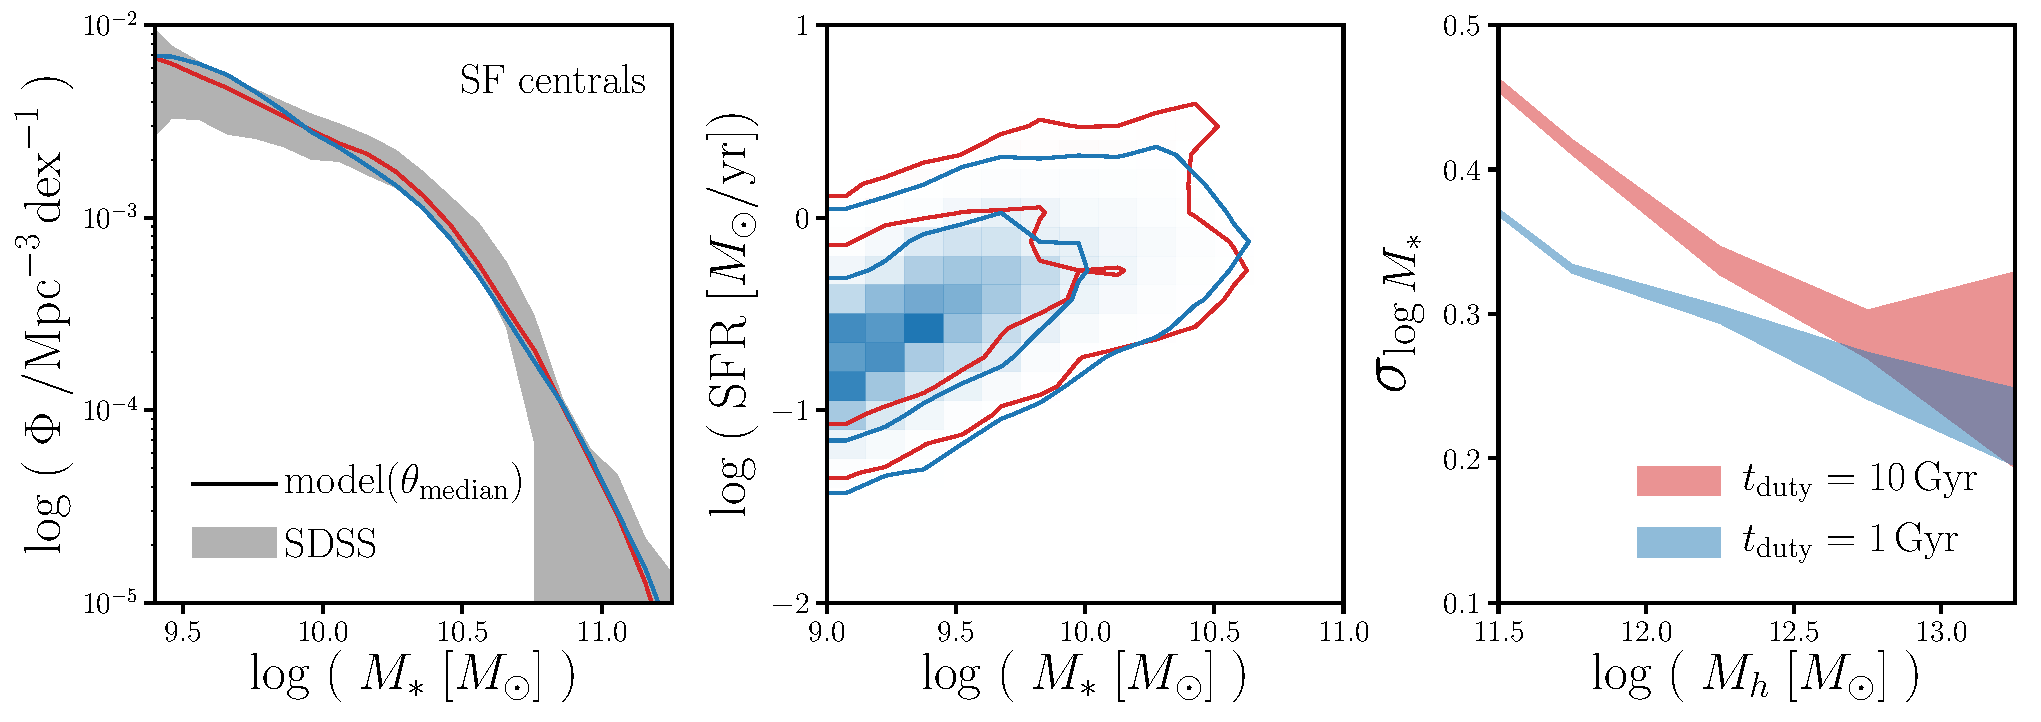
\includegraphics[width=\textwidth]{figs/qaplot_abc.pdf}
    \caption{Our models with different star formation duty cycle timescales 
    (blue: $t_\mathrm{duty}{=}1\,\mathrm{Gyr}$; red: $t_\mathrm{duty}{=}10\,\mathrm{Gyr}$) 
    run with median values of their ABC posterior distribution have SMFs and SFSs consistent 
    with observations (left and middle). \emph{They however produce significantly different 
    scatter in $\log\,M_*$ at fixed $\log\,M_\mathrm{halo}$ --- scatter in the SHMR (right)}. 
    By comparing the scatter in SHMR of our models to observational constraints on the SHMR, 
    we constrain the timescale of the star formation duty cycle and thereby the SFHs of star 
    forming galaxies.
    }
\label{fig:abc_demo}
\end{center}
\end{figure}
%%%%%%%%%%%%%%%%%%%%%%%%%%%%%%%%%%%%%

\section{Results}
Our model takes $\mathtt{TreePM}$ central subhalos and tracks their $SFR$ 
and $M_*$ evolution using a flexible parameterization of the SFS and 
SFHs that incorporate variability through a star formation duty cycle.
At $z = 0.05$, its final timestep, our model provides properties such 
as the SFR, $M_*$, and host halo mass, $M_h$, of central galaxies it 
classifies as SF. We now use these resulting properties to compare our 
model to observations and constrain its free parameters---the parameters 
of the Eq.~\ref{eq:logsfr_ms} SFS. Since the focus of our model and this 
paper is on SF centrals, the main observable we use is the SMF of star 
forming centrals in SDSS, which we estimate as 
\beq \label{eq:smf_sf_cen} 
\Phi^\mathrm{SDSS}_\mathrm{SF,cen} = f^\mathrm{cen}_\mathrm{SFS} \times f_\mathrm{cen} \times \Phi^\mathrm{Li\&White(2009)}.
\eeq
$f^\mathrm{cen}_\mathrm{SFS}$ is the fraction of central galaxies on the 
SFS, which we fit in Eq.~\ref{eq:f_cen_sfms}. $f_\mathrm{cen}$ is the 
central galaxy fraction from \cite{wetzel2013} and $\Phi^\mathrm{Li\&White(2009)}$ 
is the SMF of the SDSS from \cite{li2009}. If our model reproduces the 
observed $\Phi^\mathrm{SDSS}_\mathrm{SF,cen}$, by construction, it also 
reproduces the observed quiescent fraction. 

For the actual comparison of our model to observation, we use the parameter 
estimation framework of Approximate Bayesian Computation (ABC). ABC has the 
advantage over standard approaches to parameter inference in that it does not 
require evaluating the likelihood. It relies only on a simulation of the observed 
data and a distance metric to quantify the ``closeness'' between the observed data
and simulation. Many variations of ABC has been used in astronomy and 
cosmology~\citep[\emph{e.g.}][]{cameron2012,weyant2013,ishida2015,alsing2018}. 
We use ABC in conjunction with the efficient Population Monte Carlo (PMC)
importance sampling as in~\citep{hahn2016, hahn2017}. For initial range of our
ABC particles, \emph{i.e.} the priors of our Eq.~\ref{eq:logsfr_ms} SFS parameters
\todo{$A_z$ and $m_z$}, we use uniform distributions spanning the ranges 
\todo{numbers} and \todo{numbers}, respectively. As we mentioned in Section~\ref{sec:sfcen}, 
the range of the prior were conservatively chosen to encompass the best-fit SFS from~\cite{speagle2014} 
and measurements from~\cite{moustakas2013} and~\cite{lee2015} at $z \sim 1$. 
Finally, for our distance metric, we formulate a distance between the SMF of
the SF centrals in our model to the observed $\Phi^\mathrm{SDSS}_\mathrm{SF,cen}$ 
(Eq.~\ref{eq:smf_sf_cen}): 
\beq
\rho_\Phi = \sum\limits_{M} \left( \frac{\Phi^\mathrm{sim} - \Phi^\mathrm{SDSS}_\mathrm{SF,cen}}{\sigma'_\Phi}\right)^2.
\eeq
$\Phi^\mathrm{sim}(M)$ is the SMF of the SF centrals in our model and 
\todo{$\sigma'_\Phi(M)$ is the SMF uncertainty derived using mock catalogs from~\cite{li2009}}. 
For the rest of our ABC-PMC implementation, we strictly follow the implementation 
of \cite{hahn2017b} and~\cite{hahn2017a}. We refer reader to those papers for 
further details.

%on the right, 
%we demonstrate that different prescriptions for SFHs in our model produce significantly
%different scatter in $\log\,M_*$ for a given $\log\,M_\mathrm{halo}$ --- 
%\emph{i.e.} scatter in the SMHMR. 
%Since there are observation constraints on 
%the SMHMR, this means that we can them to better understand and constrain 
%the SFHs of star forming galaxies. 

%%%%%%%%%%%%%%%%%%%%%%%%%%%%%%%%%%%%%
% Figure 5 
%%%%%%%%%%%%%%%%%%%%%%%%%%%%%%%%%%%%%
\begin{figure}
\begin{center}
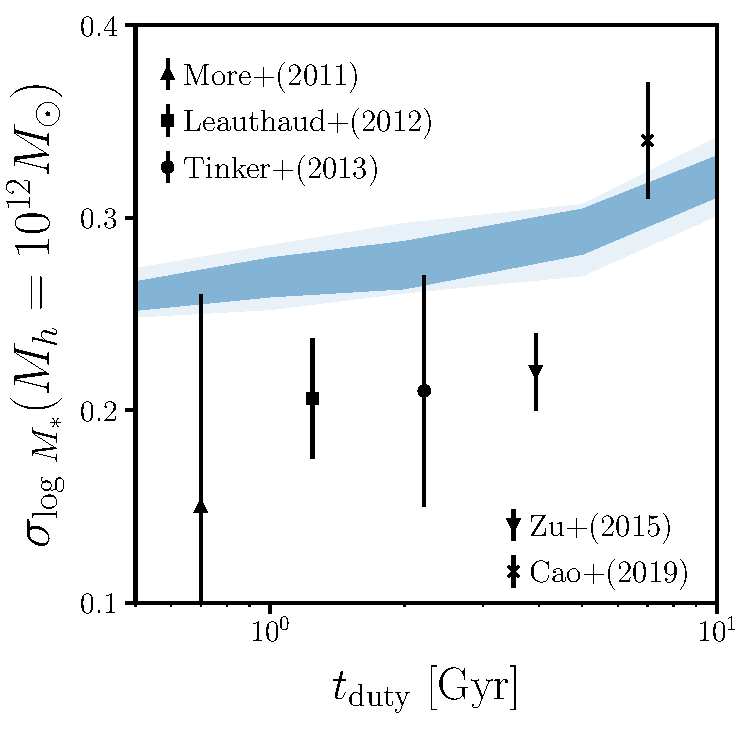
\includegraphics[width=0.75\textwidth]{figs/SHMRscatter_tduty.pdf}
    \caption{With shorter star formation duty cycle timescales, $t_\mathrm{duty}$, our model
    produces smaller scatter in the SHMR---$\sigma_{\log\,M_*}$ at $M_h{=}10^{12} M_\odot$ (left) 
    and $\sigma_{\log\,M_h}$ at $M_*{=}10^{10} M_\odot$. For $t_\mathrm{duty} = 10\,\mathrm{Gyr}$, 
    $\sigma_{\log\,M_*} = 0.32\,\mathrm{dex}$ and $\sigma_{\log\,M_h} = 0.30\,\mathrm{dex}$. 
    Meanwhile for $t_\mathrm{duty} = 0.5\,\mathrm{Gyr}$, $\sigma_{\log\,M_*}= 0.26\,\mathrm{dex}$ 
    and $\sigma_{\log\,M_h} = 0.20$. We include $\sigma_{\log\,M_*}$ 
    constraints from \cite{yang2009, more2011, leauthaud2012, tinker2013, zu2015} and 
    $\sigma_{\log\,M_h}$ constraints from~\cite{mandelbaum2006, conroy2007, more2011, velander2014, han2015} 
    (see text). The~\cite{mandelbaum2006, han2015} $\sigma_{\log\,M_h}$ constraints serve as upper limits. 
    A short star formation duty cycle timescale is necessary to produce a tight SHMR roughly
    consistent with constraints from observations. 
    }
\label{fig:sigMstar_duty}
\end{center}
\end{figure}
%%%%%%%%%%%%%%%%%%%%%%%%%%%%%%%%%%%%%
\subsection{The Star Formation Duty Cycle} \label{sec:sfdutycycle}
In Figure~\ref{fig:abc_demo}, we present the SMFs (left), SFSs (middle), and 
$\sigma_{\log\,M_*}(\mathrm{log}\,M_\mathrm{halo})$ (right) of two models 
with different SFH prescriptions each run using the medians parameter values 
of their ABC posterior distributions --- $\theta_\mathrm{median}$. One model 
has duty cycle of $t_\mathrm{duty} = 10\,\mathrm{Gyr}$ (red) while the other 
has a duty cycle of $t_\mathrm{duty} = 1\,\mathrm{Gyr}$ (blue). Both models, 
as expected from the ABC posteriors, successfully reproduce the SDSS SMF 
($\Phi^\mathrm{SDSS}_\mathrm{SF,cen}$). By construction, \emph{i.e.} the priors, 
they also have SFSs consistent with observations. Despite their consistency, 
however, \emph{the difference in the star formation duty cycle timescales of 
the models results in dramatically different scatter in $\log\,M_*$ at a given 
$\log\,M_\mathrm{halo}$ (\emph{i.e.} scatter in the SHMR)}, particularly below 
$M_\mathrm{halo} < 10^{12.5}M_\odot$. 

Since the scatter in SHMR of our model depends on the star formation duty cycle
timescale, we can compare the scatter from our model to observational constraints
on the SHMR in order to constrain the star formation duty cycle and the SFHs of star 
forming galaxies (Figure~\ref{fig:sigMstar_duty}). More specifically, in 
Figure~\ref{fig:sigMstar_duty}, we present $\sigma_{\log\,M_*}$, the scatter in 
$\log\,M_*$ at fixed halo mass, at $M_h = 10^{12} M_\odot$) and $\sigma_{\log\,M_h}$, 
the scatter in $\log\,M_h$ at fixed stellar mass, at $M_* = 10^{10} M_\odot$  
as a function of $t_\mathrm{duty}$ (left and right panels). For $t_\mathrm{duty}$ 
ranging from $10$ to $0.5\,\mathrm{Gyr}$, $\sigma_{\log\,M_*}$ ranges from 
\todo{$0.32\substack{+5.1\\ -4.0}$ to $0.26\substack{+5.1\\ -4.0}\,\mathrm{dex}$ 
and $\sigma_{\log\,M_h}$ ranges from number to number}. With a shorter star formation 
duty timescale, our model produces significantly smaller scatter in the SHMR. 

In order to constrain $t_\mathrm{duty}$, we compare $\sigma_{\log\,M_*}$ and 
$\sigma_{\log\,M_h}$ in our model to observational constraints from the 
literature. These constraints are mainly derived from fitting some sort of halo 
occupation based models to observations of galaxy clustering, SMF, satellite 
kinematics, or galaxy-galaxy weak lensing. On the left panel, we include 
$\sigma_{\log\,M_*}$ constraints from~\cite{more2011, leauthaud2012, tinker2013, zu2015}.  %yang2009, 
\cite{more2011, zu2015} fit satellite kinematics, galaxy clustering, and 
galaxy-galaxy lensing measurements of the SDSS VAGC. Meanwhile 
\cite{leauthaud2012, tinker2013} fit the SMF, galaxy clustering, and galaxy-galaxy 
lensing to COSMOS. %\cite{yang2009}, unlike the other methods, use a group catalog constructed from SDSS DR4\todo{cite} to measure the scatter in the log-normal $M_*$ distribution at a given $M_h$. 
Although, \cite{leauthaud2012, zu2015} measure 
$\sigma_{\log\,M_*}$ for all central galaxies, at $M_h\sim 10^{12}M_\odot$ there 
is a $< 1\sigma$ difference in $\sigma_{\log\,M_*}$ between star-forming and 
quiescent central galaxies~\citep{more2011, tinker2013}. Hence we 
include them in Figure~\ref{fig:sigMstar_duty}. 

\begin{comment}
    \bitem
        \item \cite{yang2009} uses a galaxy group catalog constructed from SDSS DR4 to 
            directly measure the log-normal distribution of $M_*$ at a given $M_h$.
            For blue centrals they find $\sigma_{\log\,M_*}(M_h \sim 10^{12.16}M_\odot) = 0.122 \pm 0.03$ 
            averaged over two SDSS samples and two group mass difference.

        \item \cite{more2011} uses a halo occupation based model to fit the stacked 
            velocity dispersion of satellite galaxies as a function of $M_*$ in SDSS VAGC.  
            One of the free parameters in their model is $\sigma_{\log\,M*}$, constant
            across $M_h$, for blue centrals. The best-fit model also predicts 
            $\sigma_{\log\,M_h}$ as a function $M_*$ for blue centrals. 
            
        \item \cite{leauthaud2012} joint analysis of galaxy–galaxy weak lensing, galaxy 
            spatial clustering, and galaxy number densities of the COSMOS data. 
            $\sigma_{\log\,M*}$ is constant. They get the constraint 
            $\sigma_{\log\,M_*}(M_h \sim 10^{12}M_\odot) = 0.206 \pm 0.031$ at 
            $0.2 < z < 0.48$ for all galaxies.

        \item \cite{tinker2013} uses the stellar mass function, galaxy clustering, and 
            galaxy–galaxy lensing within the COSMOS survey to constrain the stellar-to-halo 
            mass relation (SHMR) of star forming and quiescent galaxies over the redshift 
            range $z = [0.2, 1.0]$. They constrain the constant 
            $\sigma_{\log\,M_*}(M_h \sim 10^{12}M_\odot) = 0.21 \pm 0.06$ at 
            $0.22 < z < 0.48$ for star-forming galaxies.

        %\item \cite{reddick2013} constrain a model that abundance matches galaxies with the 
        %    peak circular velocity of their halos with the SDSS NYU-VAGC projected two-point 
        %    galaxy clustering and the observed conditional stellar mass functions. The model
        %    that best reproduces the data has a scatter of $0.20 \pm 0.03$ dex for all 
        %    galaxies.

        \item \cite{zu2015} 
            $\mathtt{iHOD}$: an exteded HOD model, to fit the galaxy clustering and 
            the galaxy-galaxy lensing measured from SDSS main galaxy sample and NYU-VAGC. 
            The best-fit model has $\sigma_{\log\,M_*}(M_h \sim 10^{12}M_\odot) = 0.22 \pm 0.02$ 
            for all galaxies. 
    \eitem
\end{comment}

On the right panel, we include $\sigma_{\log\,M_h}$ constraints from \cite{more2011}
along with constraints from \cite{mandelbaum2006a, conroy2007, velander2014, han2015}. 
\cite{mandelbaum2006a, velander2014} use halo occupation models to analyze galaxy-galaxy 
weak lensing measurements of SDSS and CFHTLenS\todo{cite}, respectively. 
\cite{conroy2007}, similar to \cite{more2011}, use halo model to fit the stacked 
satellite velocity disperions for SDSS VAGC. Lastly, \cite{han2015} 
use a maximum likelihood weak lensing analysis to fit shapes of SDSS source galaxies 
individually (unlike the other \emph{stacked} weak lensing analyses) for the G3Cv5 GAMA 
group catalog\todo{cite}. Each of these works ultimately measure $M_h$ in $M_*$ bins. We derive 
$\sigma_{\log\,M_h}$ from the uncertainties in these $M_h$ measurements at $M_*$ bin 
$\sim 10^{10}M_\odot$. From \cite{mandelbaum2006a, more2011, velander2014} we have 
$\sigma_{\log\,M_h}$ for blue/late-type/star forming centrals while we have 
$\sigma_{\log\,M_h}$ for all centrals for \cite{conroy2007, han2015}. 

\begin{comment}
    \bitem
        \item \cite{mandelbaum2006a} use halo occupation based model to fit SDSS galaxy-galaxy 
            weak lensing in $M_*$ bins in order to constrain the distribution of $M_h$ of 
            early/late-type centrals. 

        \item \cite{conroy2007} use halo occupation based model to fit the stacked satellite velocity
            disperions for SDSS VAGC in bins of $M_*$. For each $M_*$ bin they measure $M_h$ for 
            all central galaxies. We can convert this measurement to an upper limit on 
            $\sigma_{\log\,M_h}$.  

        %\item \cite{vanuiter2011}: weak lensing from imaging data from the $\sim 300\,\mathrm{deg}^2$ 
        %    overalp between the second Red Sequence Cluster Survey (RCS2) and SDSS DR7 using halo model 
        %    that accounts for the clustering of the lenses and distinguishes between satellite
        %    and centrals.  At $\log\,M_* = [10.0-10.5]$ $M_\mathrm{halo} = 0.56\substack{+1.66\\ -0.55}\times 10^{11}h^{-1} M_\odot$. 

        \item \cite{velander2014} conducts a stacked galaxy-galaxy weak lensing analysis
            using a HOD model on CFHTLenS data. They measure $M_h$ in bins of $M_*$ for blue/red 
            centrals at $z \sim 0.3$. We note that they correct for the scatter added from 
            the $M_*$ binning due to $M_*$ uncertainties using simulated lens and source 
            catalogs. At $< M_*> = 0.54 \times 10^10 M_\odot/h^2$ 
            $M_\mathrm{halo} = 2\substack{+0.64\\ -0.62}\times 10^{11}h^{-1} M_\odot$. 

        \item \cite{han2015} uses a maximum likelihood weak lensing analysis to fits
            shape of SDSS source galaxies individually and derive $M_h$ measurements 
            of the G3Cv5 GAMA group catalog in bins of central galaxy $M_*$. Unlike 
            the other weak lensing measurements, they do not use stacked lensing 
            measurements or a HOD model to derive the SHMR.
    \eitem
\end{comment}

%We find that by decreasing the timescale of stochasticity on a simple SFH model that traces the overall 
%SFS evolution does in fact decrease the scatter seen in the SMHMR. 
The $\sigma_{\log\,M_h}$ constraints from the literature are significantly scatter 
from $0.12$ to $0.6\,\mathrm{dex}$ (right). $\sigma_{\log\,M_h}$ from our model, 
regardless of $t_\mathrm{duty}$ is well within this range, so the comparison does 
not provide much constraint on $t_\mathrm{duty}$. Furthermore the $\sigma_{\log\,M_h}$
are not directly constrained but derived from measurements of $M_h$. On the other
hand, the constraints for $\sigma_{\log\,M_h}$ in the literature are relatively 
consistent: $\sigma_{\log\,M_*} \lesssim 0.2$. Some of these constraints are from 
analyses that use halo models that fix $\sigma_{\log\,M_*}$ as a function of 
$M_h$~\citep{leauthaud2012, tinker2013, zu2015}. Such analyses are not ideal 
measurements of $\sigma_{\log\,M_*}$ at a specific $M_h\sim 10^{12}M_\odot$.
Excluding those analyses, we are left with lower $\sigma_{\log\,M_*}$ constraints. 
These constraints are likely even lower, since observational constraints measure
the quadratic sum of the intrinsic scatter and measurement scatter. 

Based on the $\sigma_{\log\,M_*}$ comparison, we conclude that our models with 
longer duty cycles timescales produce scatters too large to reconcile with 
observations. A short duty cycle timescale, $t_\mathrm{duty} < 1\,\mathrm{Gyr}$ 
is \emph{necessary} for our model to ameliorate the tension with the constraints 
from literature. However, \emph{even for the shortest duty cycle timescale we probe 
($\sigma_{\log\,M_*} = $\todo{number} for $t_\mathrm{duty} = 0.5\,\mathrm{Gyr}$), 
we find some tension in $\sigma_{\log\,M_*}$ between our model and constraints 
in the literature.}
%\todo{talk about how observational constraints is a quadratic sum of intrinsic and measurement scatter.}  
%Tinker et al. (2017a) estimated a lower limit to the observational scatter to be 0.11 dex for their stellar masses, yielding an upper limit to the intrinsic scatter of 0.16 dex.

%%%%%%%%%%%%%%%%%%%%%%%%%%%%%%%%%%%%%
% Figure 6 
%%%%%%%%%%%%%%%%%%%%%%%%%%%%%%%%%%%%%
\begin{figure}
\begin{center}
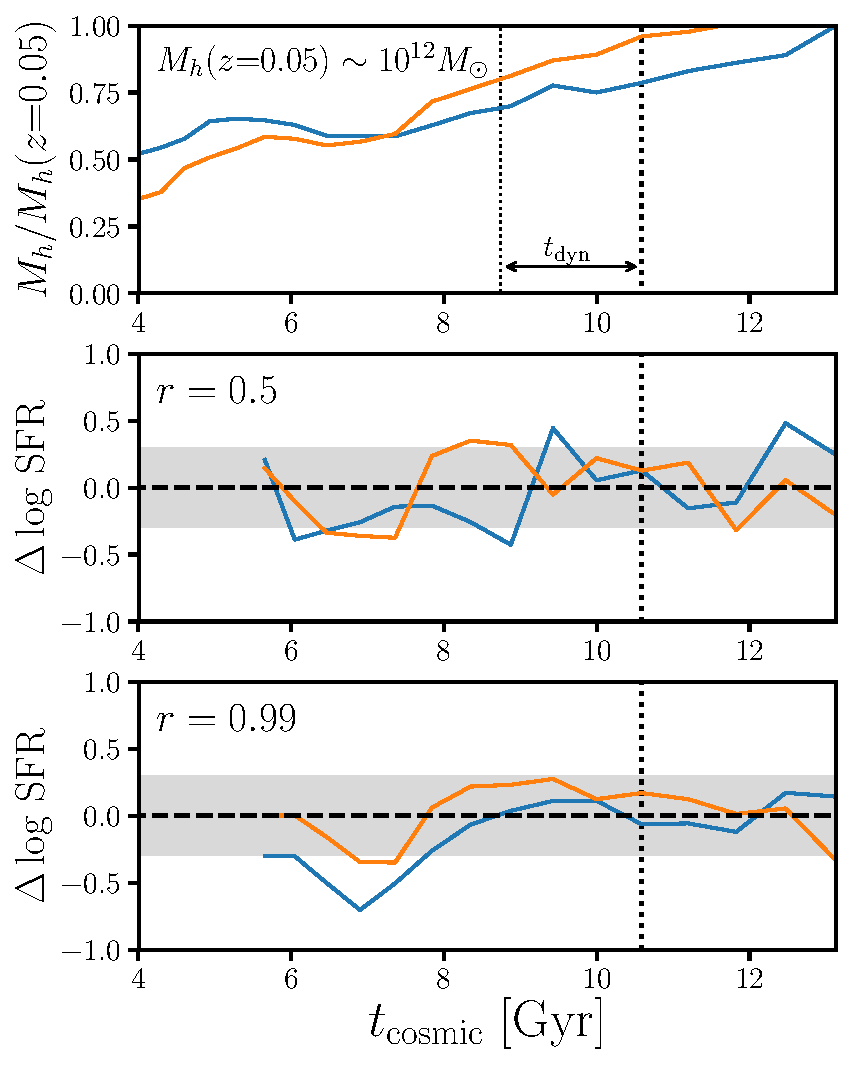
\includegraphics[width=0.5\textwidth]{figs/Mhacc_dSFR.pdf}
\caption{We incorporate assembly bias into the SF centrals of our model by 
    correlating host halo accretion history with the SFH with respect to the 
    SFS SFR. We plot the relative halo accretion history, $M_h(t)/M_h(z{=}0.05)$ 
    for two arbitrarily chosen SF centrals with $M_h(z{=}0.05)\sim10^{12}M_\odot$, 
    in the top panel. In the two panels below we present $\Delta\log\,\mathrm{SFR}$, 
    SFH with respect to the SFS, of these galaxies for our model with correlation 
    coefficients $r=0.5$ and $0.99$ (middle and bottom). At some $t$ (dotted), 
    $\Delta\log\,\mathrm{SFR}(t)$ is correlated with halo accretion over the 
    range $t - t_\mathrm{dyn}$ to $t_\mathrm{dyn}$ (shaded top panel). The 
    SFHs illustrate how $\Delta\log\,\mathrm{SFR}(t)$ correlates with 
    $\Delta M_h = M_h(t) - M_h(t-t_\mathrm{dyn})$ and with stronger correlations 
    for larger $r$.}
\label{fig:mhacc_dsfr}
\end{center}
\end{figure}
%%%%%%%%%%%%%%%%%%%%%%%%%%%%%%%%%%%%%

%%%%%%%%%%%%%%%%%%%%%%%%%%%%%%%%%%%%%
% Figure 7 
%%%%%%%%%%%%%%%%%%%%%%%%%%%%%%%%%%%%%
\begin{figure}
\begin{center}
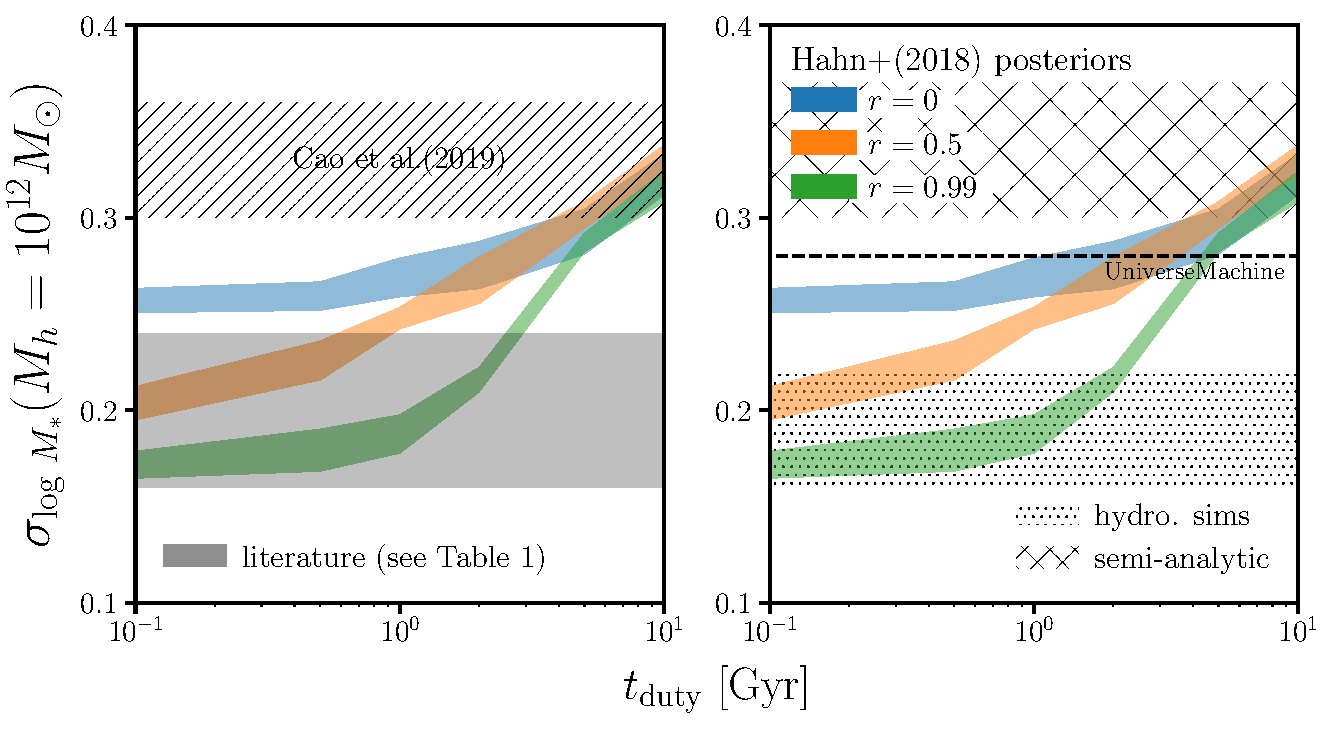
\includegraphics[width=0.75\textwidth]{figs/SHMRscatter_tduty_abias2.pdf}
    \caption{}
\label{fig:sigMstar_duty_abias}
\end{center}
\end{figure}
%%%%%%%%%%%%%%%%%%%%%%%%%%%%%%%%%%%%%
\subsection{The Need for Assembly Bias?}
A shorter star formation duty cycle timescale produces smaller scatter in the 
SHMR of our model. This dependence on the duty cycle timescale, allows us to 
compare our model with measurements of $\sigma_{\log\,M_*}$ and $\sigma_{\log\,M_h}$ 
to constrain $t_\mathrm{duty}$, which reflect the star formation variability timescale.
Such a comparisons to the literature, in the previous section, demonstrate that 
$t_\mathrm{duty} < 1\,\mathrm{Gyr}$ is necessary to reduce tensions with 
observed constraints. However, a short duty cycle timescale, alone, is not enough to 
conservatively reproduce observed $\sigma_{\log\,M_*}$ constraints. Since our model 
produces scatter in SHMR larger than observations, the SFR and $M_*$ evolution of 
the SF centrals in our model need to be more correlated with the accretion histories
of their host halos. Therefore, in an effort to better reproduce observed SHMR scatter 
constraints, in this section, we introduce \emph{assembly bias} into the SFH 
prescription of our model.

Assembly bias, most commonly in the literature, refers to the dependence of the 
spatial distribution of dark matter halos on halo properties besides 
mass~\citep{gao2005,wechsler2006,gao2007,wetzel2007,li2008,sunayama2016}.
At low halo mass, older and more concentrated halos form in high density environments. 
While at high halo mass, the effect is the opposite --- younger, less concentrated 
halos form in high-density regions. Furthermore, as predicted by semi-analytic 
models~\citep{croton2007} and found using galaxy group 
catalogs~\citep{yang2006,wang2008,tinker2011,wang2013,lacerna2014,tinker2017,tinker2017b,tinker2018},
this assembly bias propagates beyond spatial clustering to galaxy properties
such as formation histories and star formation properties. For our model, we 
incorporate assembly bias by correlating the SFHs of our SF central galaxies 
with halo growth histories. 

More specifically, we correlate the galaxy SFR with respect to the mean SFS 
SFR (\emph{i.e.} $\Delta\log\,\mathrm{SFR}$ in Eq.~\ref{eq:logsfr_sf}) to the 
halo mass accretion over dynamical time. At every $t_\mathrm{duty}$ timestep, 
$t$, $\Delta\log\,\mathrm{SFR}(t)$ is assigned based on 
$\Delta M_h(t) = M_h(t) - M_h(t - t_\mathrm{dyn}(t))$ in $M_\mathrm{max}$ bins 
with a correlation coefficient $r$, a parameter added to our model. Our 
prescription for track halo mass accretion over dynamical time is similar to 
the~\cite{rodriguez-puebla2016,behroozi2018a} empirical models. In 
Figure~\ref{fig:mhacc_dsfr} we illustrate how we incorporate assembly bias into 
the SF centrals of our model and the correlation between the host halo accretion 
history with the SFH with respect to the SFS SFR. We plot the relative halo
accretion histories $M_h(t)/M_h(z{=}0.05)$ of two arbitrarily chosen SF centrals 
with $M_h(z{=}0.05)\sim10^{12}M_\odot$ in the top panel. Below, we plot 
$\Delta\log\,\mathrm{SFR}$, SFH with respect to the SFS, of these galaxies 
for our model with correlation coefficients $r=0.5$ and $0.99$ (middle and bottom). 
At some $t$, we choose a random $\mathtt{TreePM}$ snapshot (dotted), we can see 
that $\Delta\log\,\mathrm{SFR}(t)$ is correlated with halo accretion over the 
period $t - t_\mathrm{dyn}$ to $t$ (shaded top panel). The SFHs illustrate the
correlation between $\Delta\log\,\mathrm{SFR}(t)$ and $\Delta M_h = M_h(t) - M_h(t-t_\mathrm{dyn})$
and how $\Delta\log\,\mathrm{SFR}(t)$ correlates more with $\Delta M_h(t)$ 
as $r$ ranges from $0$ to $1$ (Figure~\ref{fig:mhacc_dsfr}). 
%As an example, we mark $t$ corresponding to one of the $\mathtt{TreePM}$ snapshots in the panels (dotted) and the $t_\mathrm{dyn}$ period beforehand that we use to calculate halo accretion in the top panel (shaded). We also shade the ${\sim}1\sigma$ (${\sim}\,0.3\,\mathrm{dex}$) of the SFS SFR in the SFH panels. 

Next, using our implementation of assembly bias, we compare the model with 
different values of $r$ to observations using ABC-PMC (see Section~\ref{sec:sfdutycycle}). 
From the resulting posterior estimates, we examine the scatter in the SHMR 
($\sigma_{\log\,M_*}$) given our model %, which reproduce the observed SMF of SF centrals and SFS,
with $r=0$ (no assembly bias; blue), $0.5$ (orange), and $0.99$ (green) as a 
function of $t_\mathrm{duty}$ in Figure~\ref{fig:sigMstar_duty_abias}. We 
note that for our model run on the posterior distributions of its parameters 
reproduce the observed SMF of SF centrals and SFS, for all values of $r$.  
At $t_\mathrm{duty} \geq 5\,\mathrm{Gyr}$ we find no significant difference 
in $\sigma_{\log\,M_*}$, regardless of $r$. Below $t_\mathrm{duty} < 5\,\mathrm{Gyr}$, 
however, \emph{$\sigma_{\log\,M_*}$ of our model decreases significantly with 
stronger assembly bias in our model.} For $t_\mathrm{duty} = 0.5\,\mathrm{Gyr}$, 
we find $\sigma_{\log\,M_*} = $ \todo{final numbers} for $r = 0., 0.5$, and 
$0.99$, respectively. Comparing our updated model to the constraints included 
in Figure~\ref{fig:sigMstar_duty}, we find that incorporating assembly bias 
significantly reduces the tensions with observations (right panel). In fact, 
with a short star formation duty cycle ($t_\mathrm{duty} \leq 1\,\mathrm{Gyr}$) 
and strong assembly bias, our model conservatively reproduces most of the 
$\sigma_{\log\,M_*}$ constraints from the literature. 
%There is, however, still some tension with the \cite{yang2009} constraint: $\sigma_{\log\,M_*} = 0.122\pm0.3$. This constraint, as mentioned above, is derived using a SDSS DR4 group catalog; however, the \cite{yang2009} a number of shortcomings

In addition to the observational constraints, we also compare the SHMR scatters
of our models to $\sigma_{\log\,M_*}$ from modern galaxy formation models on the
right panel: hydrodynamic simulations (dot filled), semi-analytic models (hatched), 
and an empirial model (dashed line). For the hydrodynamic simulations, the dotted 
region encompasses constraints from EAGLE\todo{cite}, Massive Black II\todo{cite}, 
and Illustris TNG\todo{cite}, as in Figure 8 of \cite{wechsler2018}. For the 
semi-analytic models, the hatched region includes~\cite{lu2014, somerville2012}, 
and the SAGE model\footnote{\url{https://tao.asvo.org.au/tao/}}. Finally, we 
include the empirical model from \cite{behroozi2018a}, the {\sc UniverseMachine}.
By varying $r$ and $t_\mathrm{duty}$, $\sigma_{\log\,M_*}$ of our model 
encompasses all of the constraints from galaxy formation models. However, as
discussed in \cite{wechsler2018}, only the hydrodynamical simulations are in 
agreement with observations. For short $t_\mathrm{duty}$ and high $r$, $\sigma_{\log\,M_*}$ 
of our model is in good agreement with the predictions from hydrodynamic 
simulations. 

%\todo{There's not much to this figure besides the same conclusion as \cite{wechsler2018}.  Hydros are consistent with literature; SAMs and empirical models don't do so great.  In fact, our model with a short duty cycle alone (even without assembly bias) produces smaller $\sigma_{\log\,M_*}$.  }
%which traces galaxy star formation through dark matter merging histories, have somewhat larger scatter at the high mass end. This may be due to inadequate correlation betweenwhen galaxies are quenched and the properties of halos at that time; it will be important to understand what differences in the physical parameterizations lead to this difference.
A key element of our model is the SFH prescription for SF central galaxies where 
the SFH evolves about the SFS. Contrary to our SFH prescription, \cite{kelson2014}, 
for example, argue that the SFS is a simple consequence of central limit theorem 
and can be reproduced even if \emph{in situ} stellar mass growth is modeled as 
a stochastic process like a random walk. \cite{gladders2013,abramson2015,abramson2016}, 
similarly argue that $\sim2000$ loosely constrained log-normal SFHs can reproduce 
observations such as the SMF at $z \leq 8$ and the SFS at $z \leq 6$. These works, 
however, focus on reproducing galaxy observations and do not examine the galaxy-halo 
connection such as the SHMR. In order to test whether log-normal SFHs can also 
produce realistic SHMRs, we take the SFHs ($\mathrm{SFR}(t)$ and $M_*(t)$) from 
\cite{abramson2016} and assign them to halos by abundance matching their $M_*$ to 
$M_h$ at $z{\sim}1$. We then restrict the SFHs to those that would be classified as 
star-forming based on a rough $\log\,\mathrm{SSFR} > -11.$ cut. Afterwards we 
measure $\sigma_{\log\,M_*}$ at the lowest $M_h$ where it can be reliably measured 
given the \cite{abramson2016} sample $M_*{>}10^{10}M_\odot$ limit: 
$\sigma_{\log\,M_*}(M_h=10^{12.4}) = 0.33\pm0.04$ (dotted line in 
Figure~\ref{fig:sigMstar_duty_abias}). Although the \cite{abramson2016} SFHs 
can reproduce galaxy observations, $\sigma_{\log\,M_*}$ derived from the SFHs
and abundance matching have significant tension with observational constraints
and predictions from hydrodynamic simulations. This estimate is, however, 
derived from a simple abundance matching scheme. As \cite{diemer2017} find  
from their log-normal fits to the SFHs of Illustris galaxies, halo formation 
history correlates with the fits. Incorporating such assembly bias into our
abundancing matching may reduce $\sigma_{\log\,M_*}$.

In this section, we demonstrate that incorporating assembly bias into our model
by correlating $\Delta\mathrm{SFR}$ to $\Delta M_h$ reduces the tension with  
the SHMR scatter in observations. With assembly bias added, our model can 
produce the range of $\sigma_{\log\,M_*}$ constraints from observations as well as 
modern galaxy formation models. More importantly, a short star formation duty 
cycle timescale ($\lesssim 1\,\mathrm{Gyr}$) and strong assembly bias $r > 0.5$ 
is necessary to conservatively reproduce current observational constraints. 

\section{Summary and Conclusion} \label{sec:summary}


\appendix
\section{$z \sim 1$ Initial Conditions} \label{app:z1}
Much of the results presented in this paper are based on comparison 
between our model and observations at $z \sim 0.$. Our model is initalized 
at $z \sim 1$. Therefore, in this section we test some of the choices 
we make in our intializations. 

\bitem
\item Test impact of $z \sim 1$ SMF
\item Test impact of $z \sim 1$ $\sigma_{\log M_*}$ 
\eitem

%%%%%%%%%%%%%%%%%%%%%%%%%%%%%%%%%%%%%%%%%%%%%%%%%%%%%%%%%%%%%%%
% Acknowledgements
%%%%%%%%%%%%%%%%%%%%%%%%%%%%%%%%%%%%%%%%%%%%%%%%%%%%%%%%%%%%%%%
\section*{Acknowledgements}
It's a pleasure to thank 
    Louis Abramson, 
    Shy Genel, 
    \todo{more acknowledgements} 
for valueable discussions. 

\bibliographystyle{yahapj}
\bibliography{centralMS}
\end{document}
